\documentclass[aps,reprint,superscriptaddress,11pt]{revtex4-2}
\usepackage{kotex}
\usepackage[HWP]{dhucs-interword}
\usepackage[dvips]{color}
\usepackage{graphicx}
\usepackage{bm}
\usepackage{amsmath}
\usepackage{tikz}

\begin{document}
\title{응집물질물리실험 예비보고서 \\
\small 실험주제 : Crystal Growth \& X-ray diffraction,
Structure transition of BaTiO3}

\author{HuiJae-Lee}\email{hjlee6674@inha.edu}
\affiliation{Physics Department, Inha University}

\date{\today}


\begin{abstract}
이번 실험은 X-ray diffraction을 이용하여 CaTiO$_3$, SrTiO$_3$, BaTiO$_3$를 관측하고
BaTiO$_3$의 상전이를 관측하는 것을 목적으로 한다. 각 시료들은 고상소결법을 통해 제작한다.
 \end{abstract}
 
 \maketitle
 
 \section[Introduction]{Introduction}

\section[Experiment]{Experiment}
\subsection{Theory}
\subsubsection{CaTiO$_3$, SrTiO$_3$, BaTiO$_3$}

\subsubsection{고상소결법}
고상소결은 고상소결이 진행되는 공정 조건에서 모든 물질들이 고체 상태로 유지되는 공정을 의미한다.
고상소결에서는 결정립(grain)의 변화에 의해 치밀화가 발생한다. 고상소결에서는 고체-기체 계면을
고체-고체 계면으로 변환시켜 에너지를 낮추고 물질이동은 입계(grain boundary)에서 확산에 의해
발생한다.







 \subsubsection{X-ray diffraction}
X-ray diffraction는 결정 구조를 해석하는 방법 중 하나로, 브래그 법칙을 이론적인
토대로 이용한다. 결정에 X선을 입사시키면 X선의 일부는 투과하고 일부는 산란되는데
산란되는 X선은 결정 구조의 규칙성에 관한 정보를 포함한다. 규칙적으로 배열된 결정에
입사각 $\frac{\pi}{2}-\theta$로 입사하는 X선을 고려해보자(FIG~\ref{fig:bragg}).
브래그 법칙은 입사선과 평면 사이 각도 $\theta$, 결정면 사이 간격 $d$, X선의 파장 
$\lambda$ 사이 관계를 보여준다.
\begin{align}
  2d\sin{\theta} = n\lambda
\end{align}
$n$은 정수이다.

\begin{figure}[htbp]
  \centering

  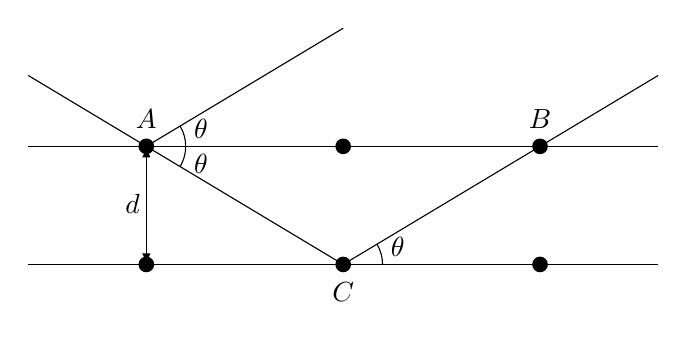
\begin{tikzpicture}
    
  \def \d {1.5}; %직선 사이 거리
  \def \x {4}; %parameter 1
  \def \y {2.5}; %점 사이 간격
  \def \t {0}; %parameter 2

  \draw (-4, \d/2) -- (4, \d/2);
  \draw (-4,-\d/2) -- (4,-\d/2);
  \draw (0,-\d/2)--(\x,  \x*\d/\y-\d/2); %C to B
  \draw (-\y,\d/2)--(\t,\d/\y*\t+3*\d/2);
  \draw (0,-\d/2)--(-\x, \x*\d/\y-\d/2); %C to A

  \node[shape=circle,fill=black,scale=0.6] at (-\y, \d/2) {};
  \draw (-\y, \d/2) node[above=3]{$A$};
  \coordinate (A) at (-\y, \d/2);
  \node[shape=circle,fill=black,scale=0.6] at ( 0, \d/2) {};
  \node[shape=circle,fill=black,scale=0.6] at ( \y, \d/2) {};
  \draw ( \y, \d/2) node[above=3]{$B$};
  \coordinate (B) at ( \y, \d/2); 
  \node[shape=circle,fill=black,scale=0.6] at (-\y,-\d/2) {};
  \node[shape=circle,fill=black,scale=0.6] at ( 0,-\d/2) {};
  \draw ( 0,-\d/2) node[below=3]{$C$};
  \coordinate (C) at ( 0,-\d/2); 
  \node[shape=circle,fill=black,scale=0.6] at ( \y,-\d/2) {};
  \draw[latex-latex] (A) -- (-\y,-\d/2) node[left=5,above=15] {$d$};
  \draw[]  (-\y+0.5, \d/2) arc(0: atan(\d/\y):0.5) 
  node[below=1,right=1.5]{$\theta$};
  \draw[]     ( 0.5,-\d/2)    arc(0: atan(\d/\y):0.5) 
  node[below=1,right=1.5]{$\theta$};
  \draw[] (-\y+0.5, \d/2) arc(0:-atan(\d/\y):0.5) 
  node[above=1,right=1.5]{$\theta$};

  \end{tikzpicture}
  \caption{결정에 입사하는 X선에 대한 브래그 법칙}
  \label{fig:bragg}
\end{figure}
\subsection{Experimental Methods}


\nocite{*}
\bibliography{ref}



%\begin{thebibliography}{9}
%\end{thebibliography}

\vfill
\end{document}